\documentclass[a4paper,10pt]{article}

\usepackage[margin=1.5cm]{geometry}
\usepackage{url}
\usepackage[numbers]{natbib}
\usepackage[dvips]{graphicx}
\usepackage{amsmath}
\usepackage{float}
\usepackage{subfigure}
\usepackage{indentfirst}
\usepackage{listings}
\usepackage{color}
\usepackage{graphicx}
%% \usepackage{nopageno}
%% \usepackage{times}

%% \usepackage{blindtext}
%% \usepackage{draftwatermark}
%% \SetWatermarkText{\underline{C}onfidential}
%% \SetWatermarkScale{4}
%% \SetWatermarkColor[gray]{0.93}

%% \pagestyle{empty}

\def\CC{{C\nolinebreak[4]\hspace{-.05em}\raisebox{.4ex}{\tiny\bf ++}}}
\def\CCT{{C\nolinebreak[4]\hspace{-.05em}\raisebox{.4ex}{\small\bf ++}}}

\definecolor{lstgray}{gray}{0.95}

\lstset{ %
  language=C++,
  captionpos=b,
  basicstyle=\footnotesize,
  %% backgroundcolor=\color{lstgray},
  %% frame=single,
  frame=tb,
  %% frameround=tttt,
  tabsize=2,
  breaklines=true,
  breakatwhitespace=false,
  numbers=left,
  %% numbersep=5pt,
  %% numberstyle=\tiny\color{lstgray},
  xleftmargin=50pt,
  xrightmargin=50pt,
  morekeywords={in,out,inout,constexpr}
}

%% \lstset{frame=L, language=C++, basicstyle=\footnotesize\ttfamily, captionpos=b, keepspaces=true, columns=flexible}

\setlength{\columnsep}{8mm}
\setlength{\parindent}{4mm}
\renewcommand{\refname}{\Large{References}}


\title{{\CCT} SG7 - Reflection\\\texttt{varid} operator}
\author{Dominic Jones\footnote{Netherhall House, London NW3 5SA, \texttt{dominic.jones@gmx.co.uk}}}
\date{\today}


\begin{document}
\maketitle


\section{Introduction}
%% A very brief high level view of your proposal, understandable by C++ committee members who are not necessarily experts in whatever domain you are addressing.

Expression tree transformations at compile-time is based exclusively on knowledge of node types. One operation, the pruning of duplicate branches, must assume that the duplicate branch is a duplicate as regards to its type \emph{and also} as regards to its actual expression. The latter is impossible to achieve cleanly without some language extension to facilitate the discrimination between different named variables of the same type used as terms in a common expression. This proposal presents a possible solution by introducing a new operator, \texttt{varid}, a function used to resolve variable identity.


\section{Motivation and Scope}
%% Why is this important? What kinds of problems does it address? What is the intended user community? What level of programmers (novice, experienced, expert) is it intended to support? What existing practice is it based on? How widespread is its use? How long has it been in use? Is there a reference implementation and test suite available for inspection?

Unique types for every terminal node, including primitive value terminals, are required when compile-time branch comparisons need to be performed. One such reason for comparing branches is to remove duplicate branches in order to avoid unnecessary repeated computation at run-time.

Consider the simple expression tree depicted in Figure \ref{fig:exprtree}. If terminal node $a$ is of type $A$, $b$ is of type $B$ and both $c_0$ and $c_1$ are of type $C$, can an equality test be correctly performed when comparing the left branch to the right branch? Presently, the answer is \emph{no}.
\begin{figure}[H]
 \centering
 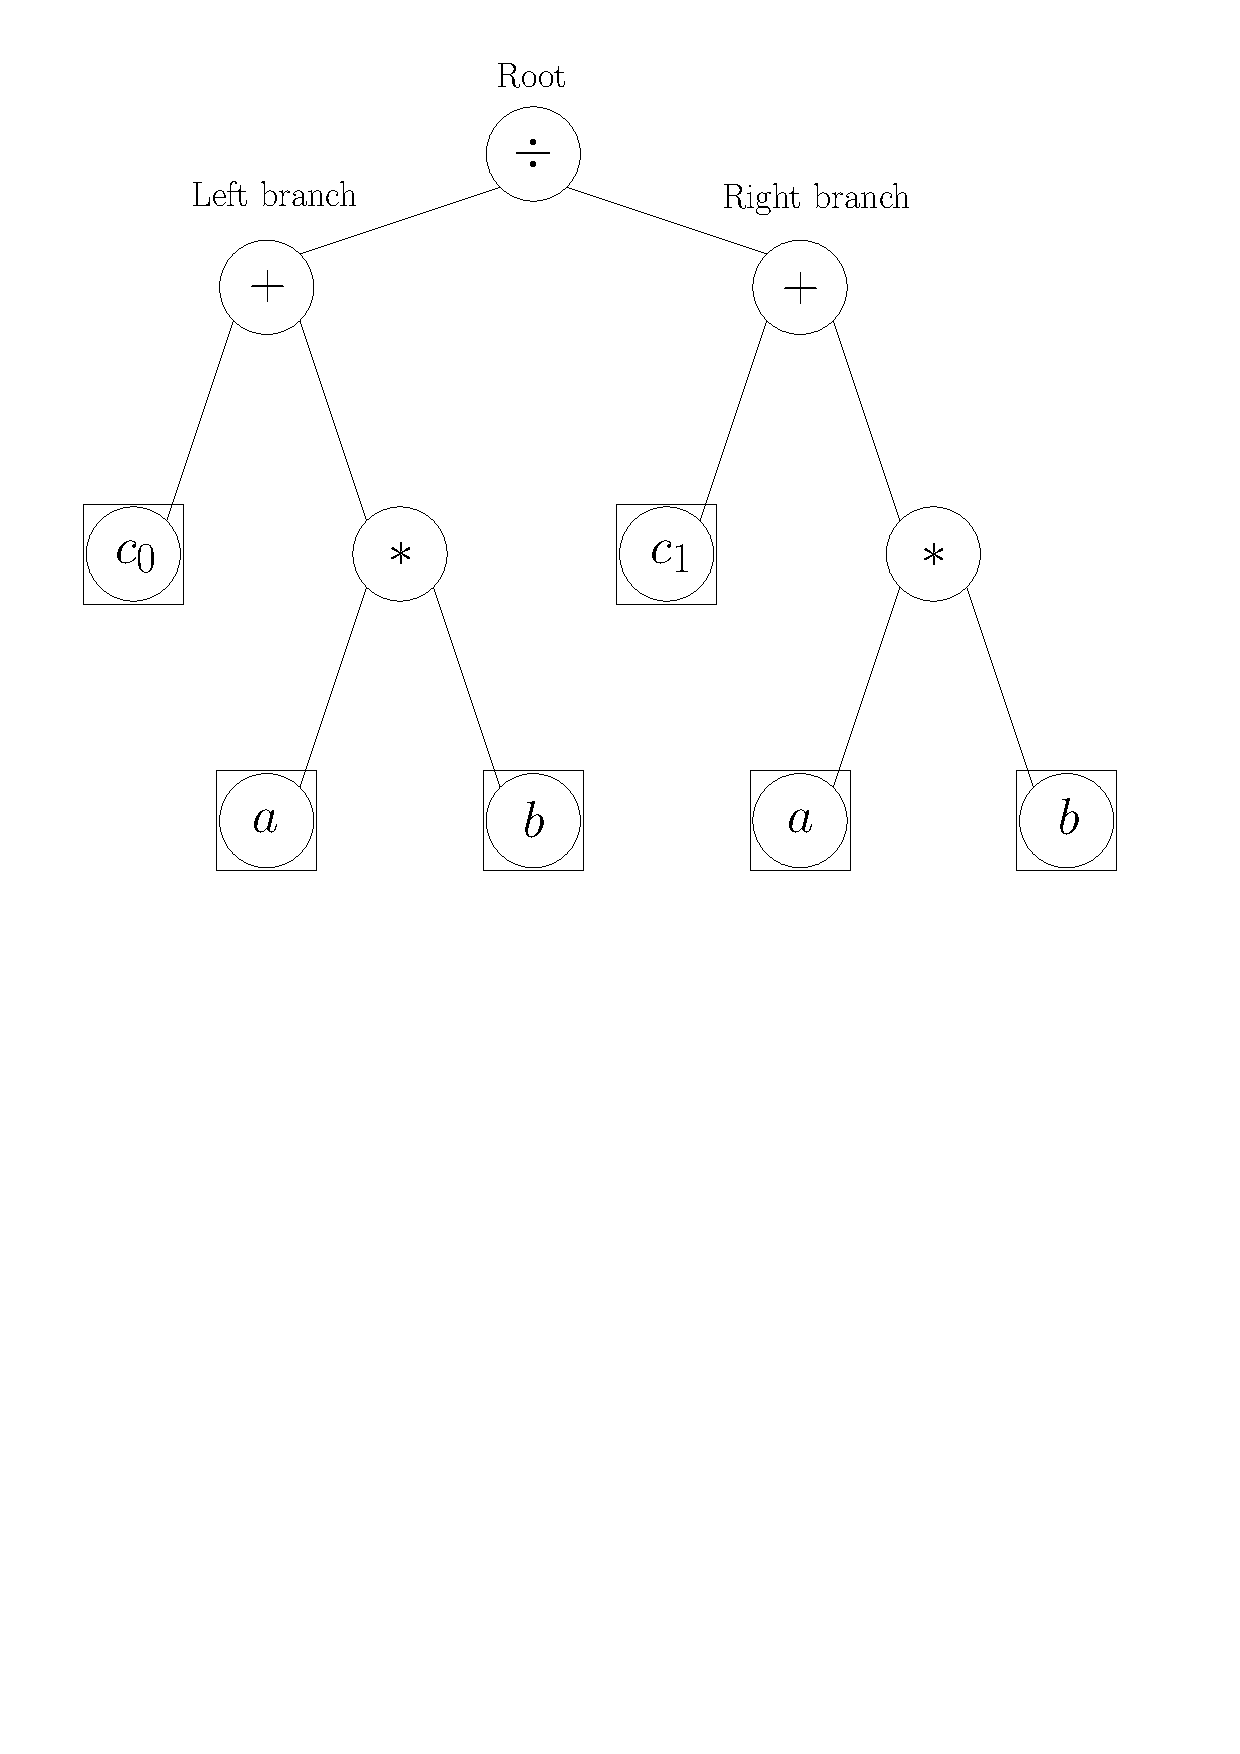
\includegraphics[width=10cm]{fig_exprtree}
 \caption{Duplicate branch? Impossible to tell given only the types.}
 \label{fig:exprtree}
\end{figure}

At compile-time, only types can be compared for equality and not memory addresses, so a problem arises when some of the terminals in the tree have a common type but in fact refer to different variables. Taking the example of Figure \ref{fig:exprtree} and assessing it in a {\CC} context (Listing \ref{lst:exprtree}), where arithmetic operators are overloaded for user-defined types to form expression types, the function would construct identical types for \texttt{t1} and \texttt{t2}, namely  \texttt{Binary<Add, double, Binary<Mul, A, B> >}. If at a later stage a duplicate branch pruning transformation was performed on the returned root of the tree, the effect would be that the root would then represent \texttt{t1 / t1}, which would be numerically incorrect.

\begin{lstlisting}[float, caption={\texttt{t1} and \texttt{t2} have the same type but do not represent the same expression.}, label=lst:exprtree]
auto evaluate(A a, B b)
{
  double c0 = 3;
  double c1 = 4;

  auto t0 = a * b;
  auto t1 = c0 + t0;
  auto t2 = c1 + t0;

  return t1 / t2;
}
\end{lstlisting}


\section{Proposal}

To provide the programmer with a means to distinguish branches that have the same type but do not represent the same expression, a small language extension is proposed to resolve this problem. In Listing \ref{lst:binary}, if a new operator was defined, \texttt{varid()}, which returned the compiler's internal index of the variable given it, and both the overloaded operators and nodes types appropriately made use of \texttt{varid()}, then the actual distinction in the expressions can be captured, enabling different branches to be distinguished \emph{and} identical branches to be matched.

Applying the change to the example in Listing \ref{lst:exprtree}, the left and right branches would become \newline \texttt{Binary<Add, double, Binary<Mul, A, B, 1, 2>, 3, 5>} and \newline \texttt{Binary<Add, double, Binary<Mul, A, B, 1, 2>, 4, 5>}, respectively. \newline Actual numbers may vary; the only point is that the generated expression types are different.

\begin{lstlisting}[float, caption={By using \texttt{varid()}, differences in expressions can be captured by incorporating the variable identity in the host node type.}, label=lst:binary]
template<typename Fn, typename L, typename R,
         std::size_t IL, std::size_t IR>
struct Binary
{
  Binary(L const &l, R const &r);
  ...
};

template<typename L, typename R>
auto operator+(L const &l, R const &r)
-> Binary<Add, L, R, varid(l), varid(r)>
{
  return {l, r};
}
\end{lstlisting}


\section{Design Decisions}
The proposed feature can be emulated to a certain degree by wrapping variables of the same type but different value in a host class, whose type is in some way unique. Listing \ref{lst:exprtreealt} presents a work-around to solving the problem in Listing \ref{lst:exprtree}, but is far from ideal as it relies on existing non-standard functionality and forcing the programmer to use an awkward syntax.

\begin{lstlisting}[float, caption={\texttt{\_\_COUNTER\_\_} could be used as a mechanism to generate unique types.}, label=lst:exprtreealt]
template<std::size_t ID, typename T> struct Unique { T value; };

#define UQ(value) Unique<__COUNTER__, decltype(value)>{value}

auto evaluate(A a, B b)
{
  double c0 = 3;
  double c1 = 4;

  auto t0 = a * b;
  auto t1 = UQ(c0) + t0;
  auto t2 = UQ(c1) + t0;

  return t1 / t2;
}
\end{lstlisting}

\section{Technical Specifications}

\texttt{varid} takes one argument which must be a named variable or reference and returns the compiler-specific index of the variable, of type \texttt{std::size\_t}. The operator name would introduce a new keyword into the language.

\begin{lstlisting}[caption={Valid uses of \texttt{varid}}, label=lst:vaild]
double c0 = 3;
double c1 = 4;
static_assert(varid(c0) != varid(c1));

auto &cr = c0;
static_assert(varid(cr) == varid(c0));

cr = c1;
static_assert(varid(cr) == varid(c1));
\end{lstlisting}


\begin{lstlisting}[caption={Invalid uses of \texttt{varid}}, label=lst:invalid]
double c0 = 3;
double c1 = 4;
auto conexpr i0 = varid(c0 * c1); // error: expressions not supported
auto conexpr i1 = varid(3);       // error: literals not supported
auto conexpr i2 = varid(double);  // error: types not supported
\end{lstlisting}


\section{Technical Issues}
In the case of temporary variables (Listing \ref{lst:exprtreetmp}) being passed to the overloaded operator functions as \texttt{const} qualified references (Listing \ref{lst:binary}), ideally the returned value of \texttt{varid} should be related to the temporary that was passed, i.e. associated to the scope from where the temporary was received rather than the local scope of the function itself. This, however, may be a difficult requirement to achieve.

\begin{lstlisting}[caption={\texttt{c0} and \texttt{c1} (from Listing \ref{lst:exprtree}) are now replaced by literals, but this should not effect the generated types of \texttt{t1} and \texttt{t2}.}, label=lst:exprtreetmp]
auto evaluate(A a, B b)
{
  auto t0 = a * b;
  auto t1 = 3.0d + t0;
  auto t2 = 4.0d + t0;

  return t1 / t2;
}
\end{lstlisting}


%% \bibliographystyle{plainnat}
%% \bibliographystyle{unsrt}
%% \bibliography{references,publications}
\end{document}
